\documentclass[12pt]{article}
\usepackage[english]{babel}
\usepackage{natbib}
\usepackage{url}
\usepackage[utf8x]{inputenc}
\usepackage{amsmath}
\usepackage{graphicx}
\graphicspath{{images/}}
\usepackage{parskip}
\usepackage{fancyhdr}
\usepackage{vmargin}
\usepackage{float}
\usepackage{hyperref}
\setmarginsrb{2 cm}{1.5 cm}{2 cm}{1.5 cm}{1 cm}{1.5 cm}{1 cm}{1.5 cm}

\title{Analysis of NHIS(National Health Interview survey) data and building associated software components}	
\author{Ankitha Kumari Moodukudru\\
Deepanshu Parihar\\
Harish Ramani\\
Viral Pandey}% Author
\date{\today}											% Date

\makeatletter
\let\thetitle\@title
\let\theauthor\@author
\let\thedate\@date


\pagestyle{fancy}
\fancyhf{}


\begin{document}

%%%%%%%%%%%%%%%%%%%%%%%%%%%%%%%%%%%%%%%%%%%%%%%%%%%%%%%%%%%%%%%%%%%%%%%%%%%%%%%%%%%%%%%%%

\begin{titlepage}
	\centering
    
    
\includegraphics[scale = 0.75]{logo.jpg}\\[1.0 cm]	% University Logo
   
	\textsc{\Large DS5110}\\[0.5 cm]				% Course Code
	\textsc{\large Introduction to Data management and Processing}\\[0.5 cm]				% Course Name
	\rule{\linewidth}{0.2 mm} \\[0.4 cm]
	{ \huge \bfseries \thetitle}\\
	\rule{\linewidth}{0.2 mm} \\[1.5 cm]
	
	\begin{minipage}{0.4\textwidth}
		\begin{flushleft} \large
		
			\theauthor
			\end{flushleft}
			\end{minipage}~
			\begin{minipage}{0.4\textwidth}
		
	\end{minipage}\\[2 cm]
	

 
	\vfill
	
\end{titlepage}

%%%%%%%%%%%%%%%%%%%%%%%%%%%%%%%%%%%%%%%%%%%%%%%%%%%%%%%%%%%%%%%%%%%%%%%%%%%%%%%%%%%%%%%%%

\tableofcontents
\pagebreak

%%%%%%%%%%%%%%%%%%%%%%%%%%%%%%%%%%%%%%%%%%%%%%%%%%%%%%%%%%%%%%%%%%%%%%%%%%%%%%%%%%%%%%%%%

\section{Summary}
The National Health Interview Survey (NHIS) is a yearly cross-sectional household interview survey conducted by the Centers for Disease Control and Prevention’s National Center for Health Statistics. Data is collected from a selected sample of households in US by conducting face to face interviews. The survey contains data related to demographics, health status and limitations, injuries, health care access and utilization, health insurance, income and assets.
The data set contains responses from seven questionnaires corresponding to household, family, child, injury and disability data. We wanted to explore the following aspects of the data set: 
\begin{itemize}
\item Compare the mental health of individuals who practice meditation and other    relaxation techniques 
\item Identify factors affecting sleep quality among the participants
\item The Affordability of health care and deficiency aiding devices 
\item Consider the scenario where a business owner wants to explore the data but he/she relies on people with programming skills to help  answer important questions. A more intuitive approach would be for the owner to ask what he/she wants as a text query to a bot and get all the visualizations. In this project, we have exposed the NHIS dataset via a conversational bot and suggest frameworks by which this could be generalized for any dataset.
\end{itemize}

We analyzed the data from adults of the age 18 years and above who participated in the NHIS survey of 2017. 

\section{Methods}

\subsection{Analysis of effect of yoga and meditation on emotional well-being:}

The survey consisted of user responses that were marked uncertain, not mentioned and refused. These observations were filtered out for the selected columns as they did not favor the analysis.
Participants' self-reported feelings were captured using a set of 6 questions, each one corresponding to feelings such as sad, nervous, fidgety, worthless, everything required effort and hopeless. Each of these variables contained 5 levels representing the frequency of occurrences of these feelings. Participants' response to practice of yoga or meditation was scattered across multiple columns, each one corresponding to a specific technique of meditation, yoga, tai chi etc.    

The variables for yoga and meditation were merged into 2 variables by performing a logical OR on the responses for individual practices. 
In order to capture the overall psychological distress level of a participant the variables related to feelings were merged into a negative emotion score, that ranged from 0 to 1.  This variable was used to visualize the distribution of distress levels in the yoga and meditation practicing groups.
We also analyzed the frequency of experiencing these feelings with yoga and meditation by employing the chi-square test of independence with a significance level set at P $<$ 0.05.


\subsection{Analysis of quality of sleep and the contributing factors:}
The survey consisted of responses on the self reported hours of sleep and other associated attributes such as sleep medication. We collated these columns into one sleep score so that we can compare it with other factors. We weighed all these variables differently and came up with sleep score as follows:

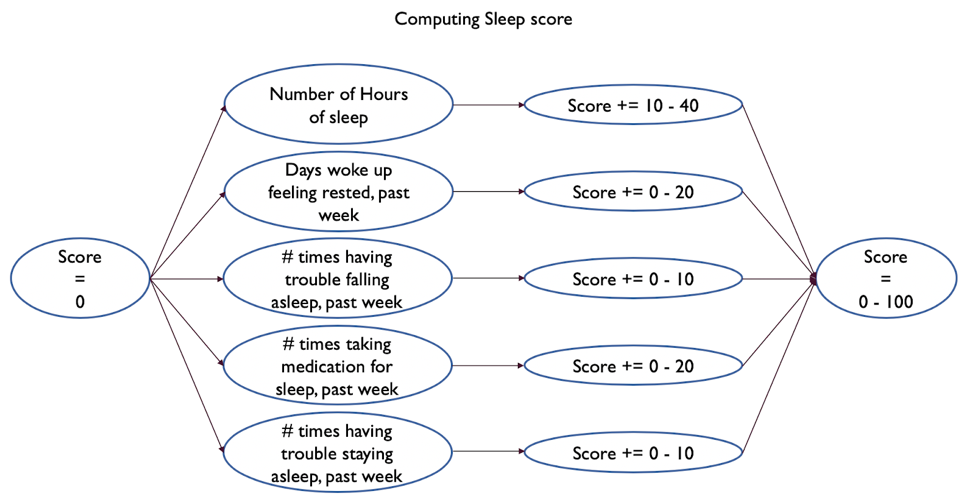
\includegraphics[scale = 0.75]{sleepscore.png} 

Then, based on the initial analysis we chose 60 variables out of the available variables. We plotted them with the sleep score that we devised to check for any linear patterns. We got 23 such variables which showed linear relationship with sleep score. 
After fitting the linear model with them and plotting the residuals of it with the variables, We chose these variables as predictor variables:\\
\begin{itemize}
    \item PHSTAT:     How would you describe your health in general?
    \item ASIMEDC: How worried are you right now about not being able to pay medical costs of a serious illness or accident?
    \item ASICNHC:  How worried are you right now about not being able to pay medical costs for normal health care?
    
\end{itemize}
We did cross k fold validation with 10 partitions to check the accuracy of the model.\\

\subsection{Analysis of affordability of health care}
Based on the survey responses, we came across certain measures to detect affordability of dental care and eyeglasses. So we defined a new feature called affordability which could represent the affordability of the two responses as one . This feature has values 0,1 or 2 based on the person’s ability to afford neither , one or both of eyeglasses and dental care.
Then, we narrowed the number of factors affecting affordability by going through the code book and filtering out columns related to vision and dental care for building the model. 
As the classes we were trying to predict were more than two,  we tried a multinomial logistic regression algorithm to fit a model based on Age-Group , medical bills and relative coverage compared to a year ago.
The challenge we faced was of data imbalance [Figure \ref{fig:dataimbalance}] as observations for one class was dominating the other two after omitting all rows with missing values in them. This was solved using the upsample function of caret package which replicates previous observations of minority class to build new values to obtain data balance [Figure \ref{fig:databalance}].
\subsection{Conversational Bot}
A conversational bot was developed using slack as the interface and dialogflow for processing the texts entered by the user as represented in [Figure \ref{fig:arch}]
The components of the bot are as follows:
\begin{itemize}
    \item Slack – It is a popular cloud based set of propriety team collaboration tools and services. We use it to create a bot through which we can deliver all the needs of the business owner to visualize and interpret his data by asking questions in natural language.
    \item Dialogflow – It is a google owned technology that gives a framework for processing natural language.
    Important terminologies in dialogflow :
\begin{itemize}
\item Entity:  Keywords that are specific to a particular application. In our bot, all the names of the columns of the data are specific to our application and they can be treated as entities. 

\item Intent: They are basically to match what the user wants. We can create intents by giving some training examples and if the user input matches the common underlying pattern, the intent is triggered. It can be used to parse user texts in a structured manner and get the desired entities.

\item Fulfillment:  A separate service or a url could be triggered once an intent is matched. It is called a fulfillment service. In our application, we write our own service and configure the url in dialogflow.
\end{itemize}
\item Application Layer – It is a node server which is the backend for the entire application. It handles requests from slack, and calls dialogflow and parses the response for it to be viewed in slack.
\item Data Layer:  It is where the R scripts reside that produces the visualization . The visualizations are then put to an S3 bucket and the link is returned back to the user. All the scripts are exposed as an API (Application Programmable Interface ) via Plumber package. All the cleaned data from the analysis are exported in a R package that was created especially for this purpose. 
\item Workflow: [Figure \ref{fig:bot}]
\end{itemize}

\section{Results}

\subsection{Analysis of effect of yoga and meditation on emotional well-being:}
\begin{itemize}
\item 16\%\ of the US population engage in meditation and a majority of them practice spiritual meditation.

\item 24 \%\ of the US population experience psychological distress of some level.  And most of them reported feeling nervous and fidgety more often. 
   
    \item The negative emotion score was plotted against yoga and meditation separately to analyze the distribution of frequencies of emotion scores in each of these categories. It was observed that more participants had higher psychological distress level in the non-yoga and non-meditation participating groups [Figure \ref{fig:yoga}] and [Figure \ref{fig:meditation}]
    
    \item The chi square test between the frequency of feelings reported vs meditation and yoga (separate), returned a very low p-value, confirming that they are related. [Figure \ref{fig:frequency}] and [Figure \ref{fig:chisq} ]
\end{itemize}
 
\subsection{Analysis of quality of sleep and the contributing factors:}
On performing exploratory analysis on the data set, the following results were observed:
\begin{itemize}
    \item We found that people who where financially stable such as having regular income from salary or other sources slept healthy amount of hours compared to others who were financially unstable [Figure \ref{fig:sleepvsincome}]. 
    \item Only 62\% of the United States population sleeps for healthy amount of hours on an average. i.e. between 7 and 9 hours.
    \item Nearly 14\% of the population sleeps for unhealthy amount of hours i.e. less than 6 hours or more than 10 hours.
\end{itemize}

The Sleep score devised using the sleep information was plotted with other variables in the data set giving interesting results about the correlation between them. For example,
\begin{itemize}
    \item Factors such as marital status was correlated with the sleep score. People who were married had a better sleep score than people who were either divorced, widowed or separated.
    \item We found correlation between the citizenship status of an individual and his/her sleep score.
    \item Health was strongly correlated with the sleep score. Individuals who felt their health was excellent had way better sleep score than people who thought otherwise [Figure \ref{fig:sleepvshealth}].
    \item Financial conditions like the affordability of medical costs for emergency or normal health care was strongly correlated with sleep score. People who were worried about these costs had lower sleep score than others [Figure \ref{fig:sleepvshealthcare}].
\end{itemize}

By choosing the appropriate predictor variables based on the analysis and linearity patterns, we fitted a linear model which can predict a sleep score based on the input values for the predictor variables. The model has a test RMSE of 18.83

\subsection{Analysis of affordability of health care}
\begin{itemize}
    \item 80\% of the survey takers were insured while 20\% were uninsured.[Figure \ref{fig:insurance}]
    \item Private plans were the most used among all health care insurance plans.[Figure \ref{fig:privateplans}]. In those plans PPO (employer -provided health insurance) plans dominated all others.[Figure \ref{fig:ppo}]
    \item The people under PPO plans were not confident in their ability to find affordable health care plans on their own. [Figure \ref{fig:notconfident}]
    \item High costs and  loss of job/change of employers were the leading factors for being uninsured in the past year.[Figure \ref{fig:notinsured}]
    \item Among people facing vision issues 90\% had their current status of visibility as chronic.[Figure \ref{fig:visibility}]
    \item Change in health care plans had no effect on affordability of either eyeglasses or dental care.
    \item There was no linear decrease in either eyeglasses or dental care being not affordable with increasing income levels.[Figure \ref{fig:eyeglass}]
\end{itemize}

\subsection{Conversational Bot}

Sample screen shot of the slack bot as referred in [Figure \ref{fig:slack}]

\section{Discussion}
\subsection{Analysis of effect of yoga and meditation on emotional well-being:}
\begin{itemize}
    \item The US population is adopting yoga, meditation and associated practices along with being engaged in regular physical activities.
    \item The data did not contain sufficient information to study the impact of yoga or meditation on the behavioral health.In order to further understand the effect, we need to design an experiment targeted at how often they have been practicing meditation/yoga and also track their feelings over a period of time.
    \end{itemize}
     \subsection{Analysis of quality of sleep and the contributing factors:}
    \begin{itemize}
   \item We expected factors such as smoking and alcohol habits to impact the sleep quality, but the data in hand did not show any such correlation. 
   \end{itemize}
   \subsection{Analysis of affordability of health care}
   \begin{itemize}
   
    \item 80\% of the US population is insured under some type of health care which is different from developing countries. Also the transition from one health plan to another is smooth and doesn’t cause people much trouble in paying bills.
    \item The number of people who could afford both eyeglasses and dental care were much more than the other two which shows that they are generally affordable or that the distribution of survey  is not even across different sections of the population.
    \item People with employment need to be taught about finding health insurance so that they feel more confident in finding one as loss of job is one of the major reasons for being uninsured.
    \item To improve the results, we will try to find more data which could probably give us more observations for cases where affordability has values of 0 and 1. This would help us to build a better predictive model and  also solve the issue of data imbalance. While doing this we can also come across more features that can be used as explanatory variables.
    \end{itemize}
    \subsection{Conversational Bot}
\begin{itemize}
    \item To make it usable for any data we need every data to be structured the same way (Which is nearly impossible) or have an utility that parses the code book info to generate metadata.  A sample meta data file can contain these information. 
    \begin{itemize}
    

    \item Description of the whole data set.
    \item A set of tags that describe the data set. This can be used to merge two data sets or columns together in the future.
    \item Description for each column.
    \item A set of tags from the corpus that describe the column.
    \item Data type for each column.
    \item Any special values that indicate NA.
    \item Levels if its a categorical column.
    
\end{itemize}

\end{itemize}


\section{Statement of Contribution}
Ankitha Kumari Moodukudru: Performed analysis of yoga, meditation and feelings variables. Wrote functions and added metadata in the R package corresponding to the analysis performed. 

Deepanshu Parihar: Responsible for the analysis of health insurance aspect of the data. Built a predicitive model for affordability of dental care and eyeglasses. Added functions and metadata in the R package for the data related to healthcare.

Harish Ramani: Responsible for creating the conversational bot. Participated in the initial exploratory analysis of the data. Created the initial R package structure and maintained the whole project by reviewing pull requests and adhering to best practices.

Viral Pandey: Responsible for analysis of sleep patterns and associated factors affecting the sleep quality of the participants. Built a linear model that predicts sleep score of an indivual. Added functionality and metadata corresponding to the analysis in the R package.

\section{References}
\begin{itemize}
\item \href{https://www.cdc.gov/nchs/nhis/index.htm}{NHIS Raw Data}
\item \href{https://dialogflow.com/docs}{Dialogflow documentation}
\item \href{https://www.rplumber.io/docs/}{Plumber API Documentation}
\item \href{https://hilaryparker.com/2014/04/29/writing-an-r-package-from-scratch/}{R Package tutorial}

\end{itemize}


\newpage

\section{Appendix}
\subsection{Links}
\begin{itemize}
\item \href{https://github.com/mancunian1792/nhis5110}{R Package}
\item \href{https://github.com/mancunian1792/nhis_chatbot}{Chat Bot}
\item \href{https://www.youtube.com/watch?v=zpw6n1dUXuQ&feature=youtu.be}{Chat Bot Demo}


\end{itemize}
\subsection{Images}
\begin{figure}[H]
\centering
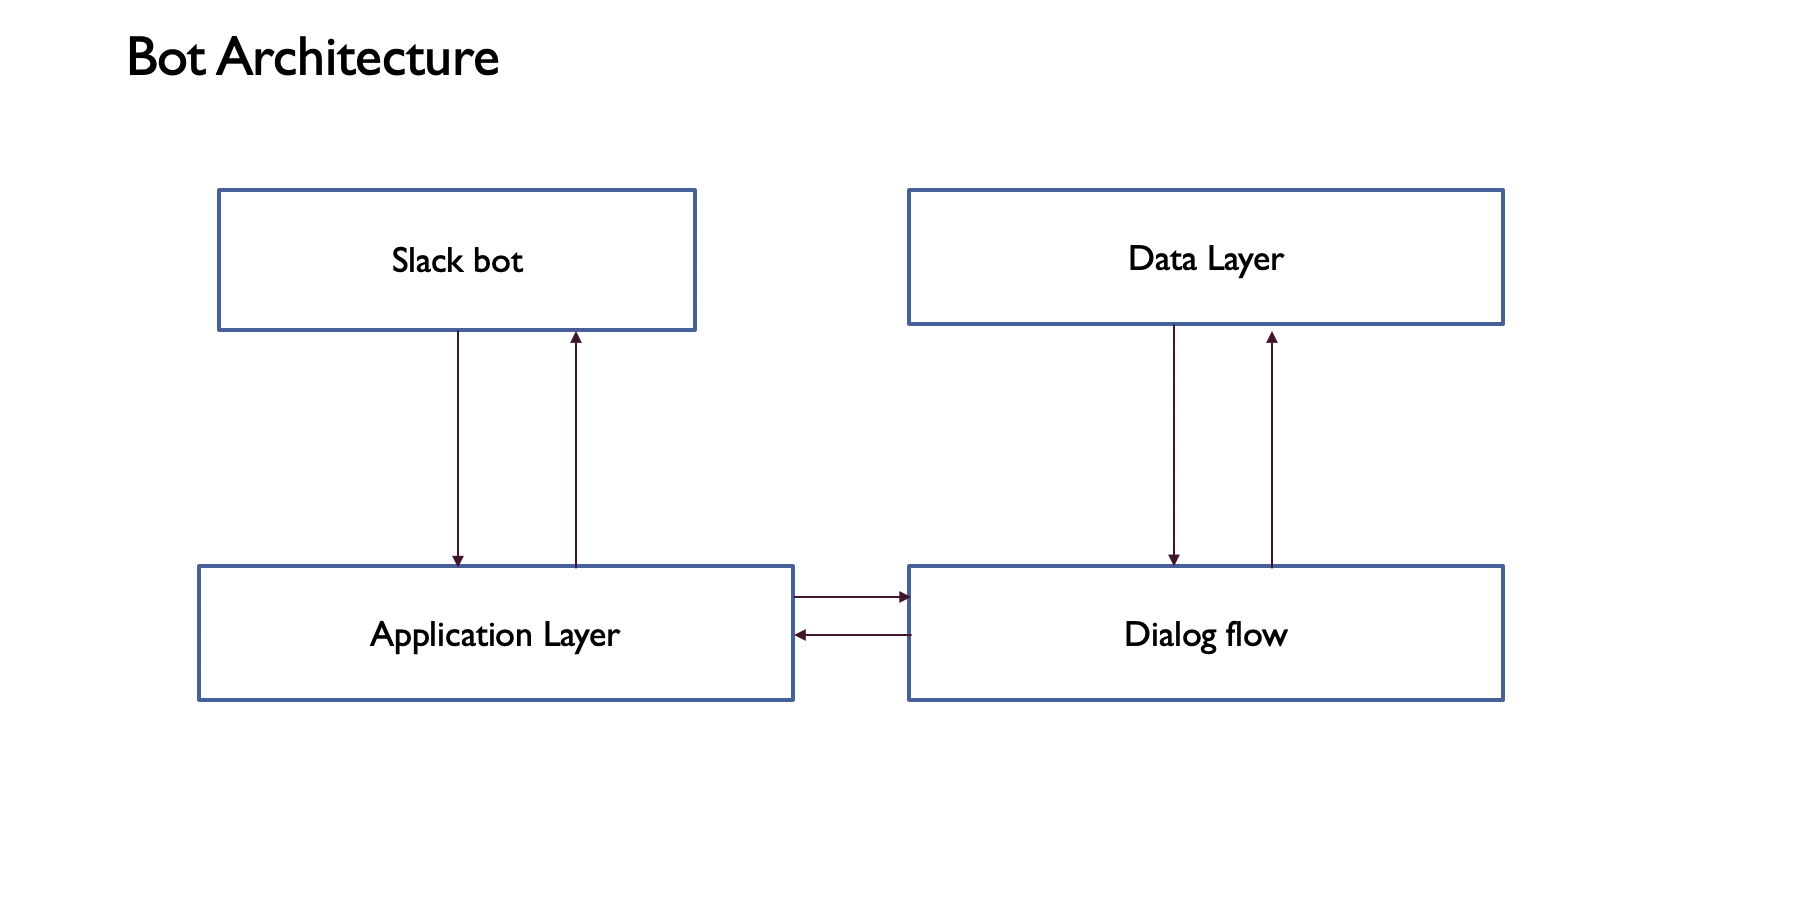
\includegraphics[scale = 0.5]{architecture.png}
\caption{Bot Architecture}
\label{fig:arch}
\end{figure}

\begin{figure}[H]
\centering
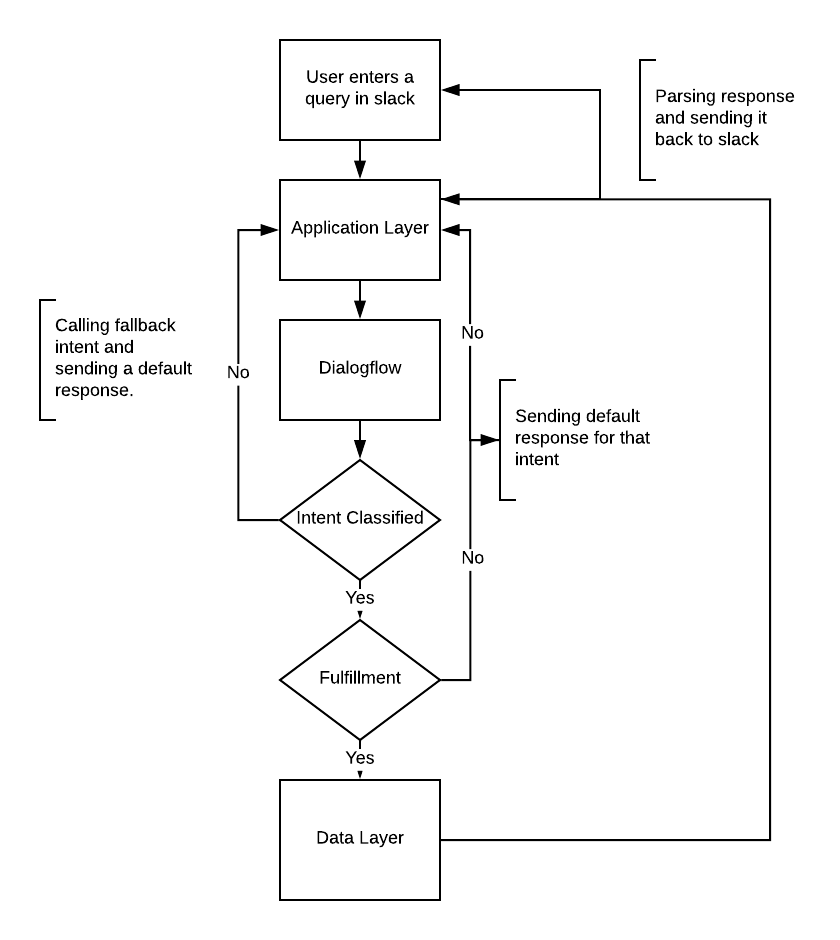
\includegraphics[scale = 0.5]{botflowchart.png}
\caption{Flow chart for Bot}
\label{fig:bot}
\end{figure}


\begin{figure}[H]
\centering
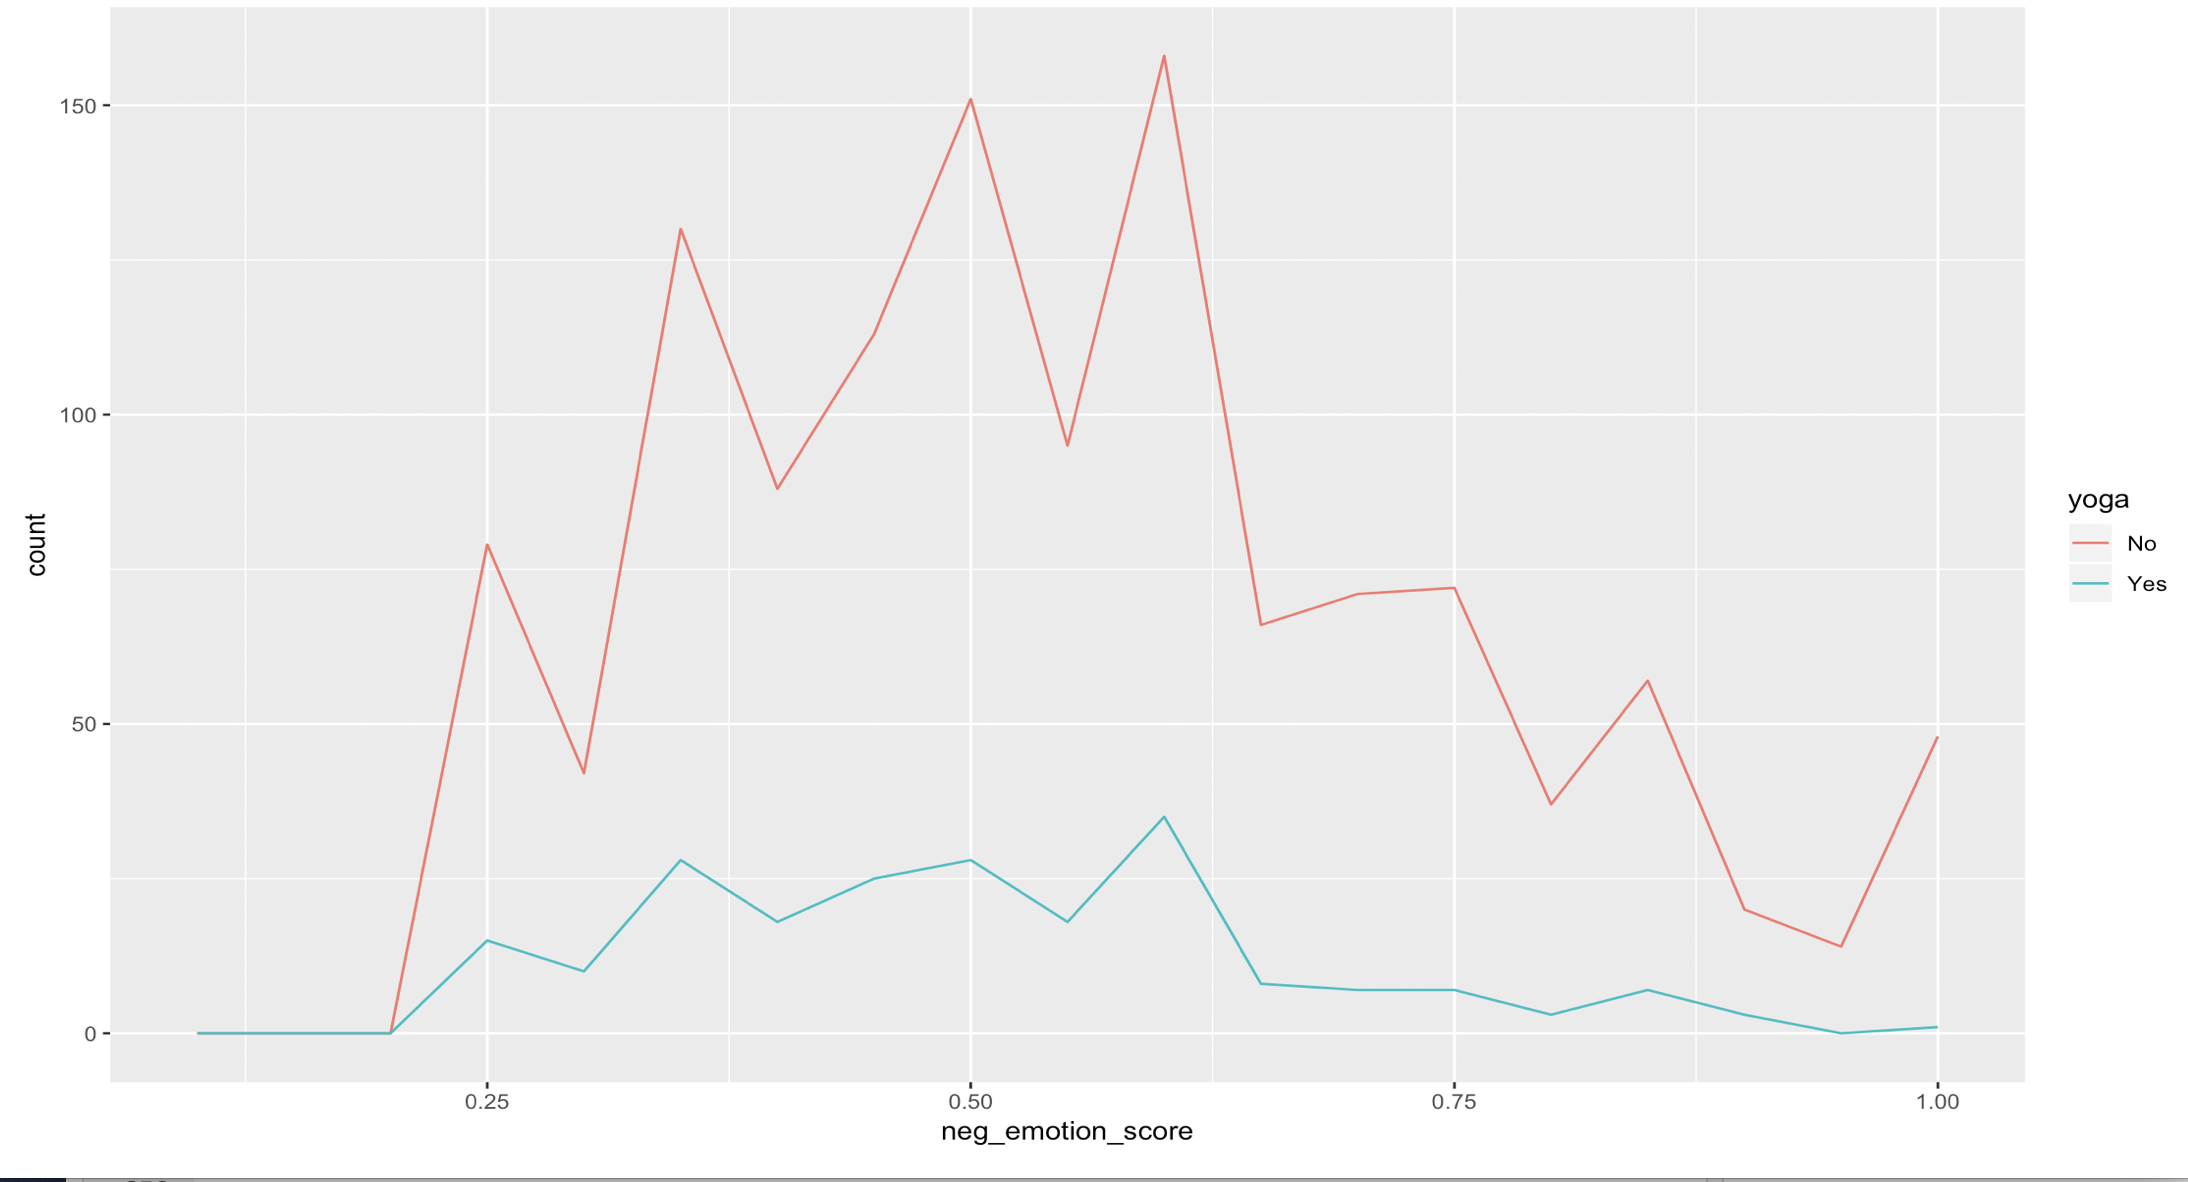
\includegraphics[scale = 0.4]{yogascore.png}
\caption{Yoga Vs Negative emotion score}
\label{fig:yoga}
\end{figure}

\begin{figure}[H]
\centering
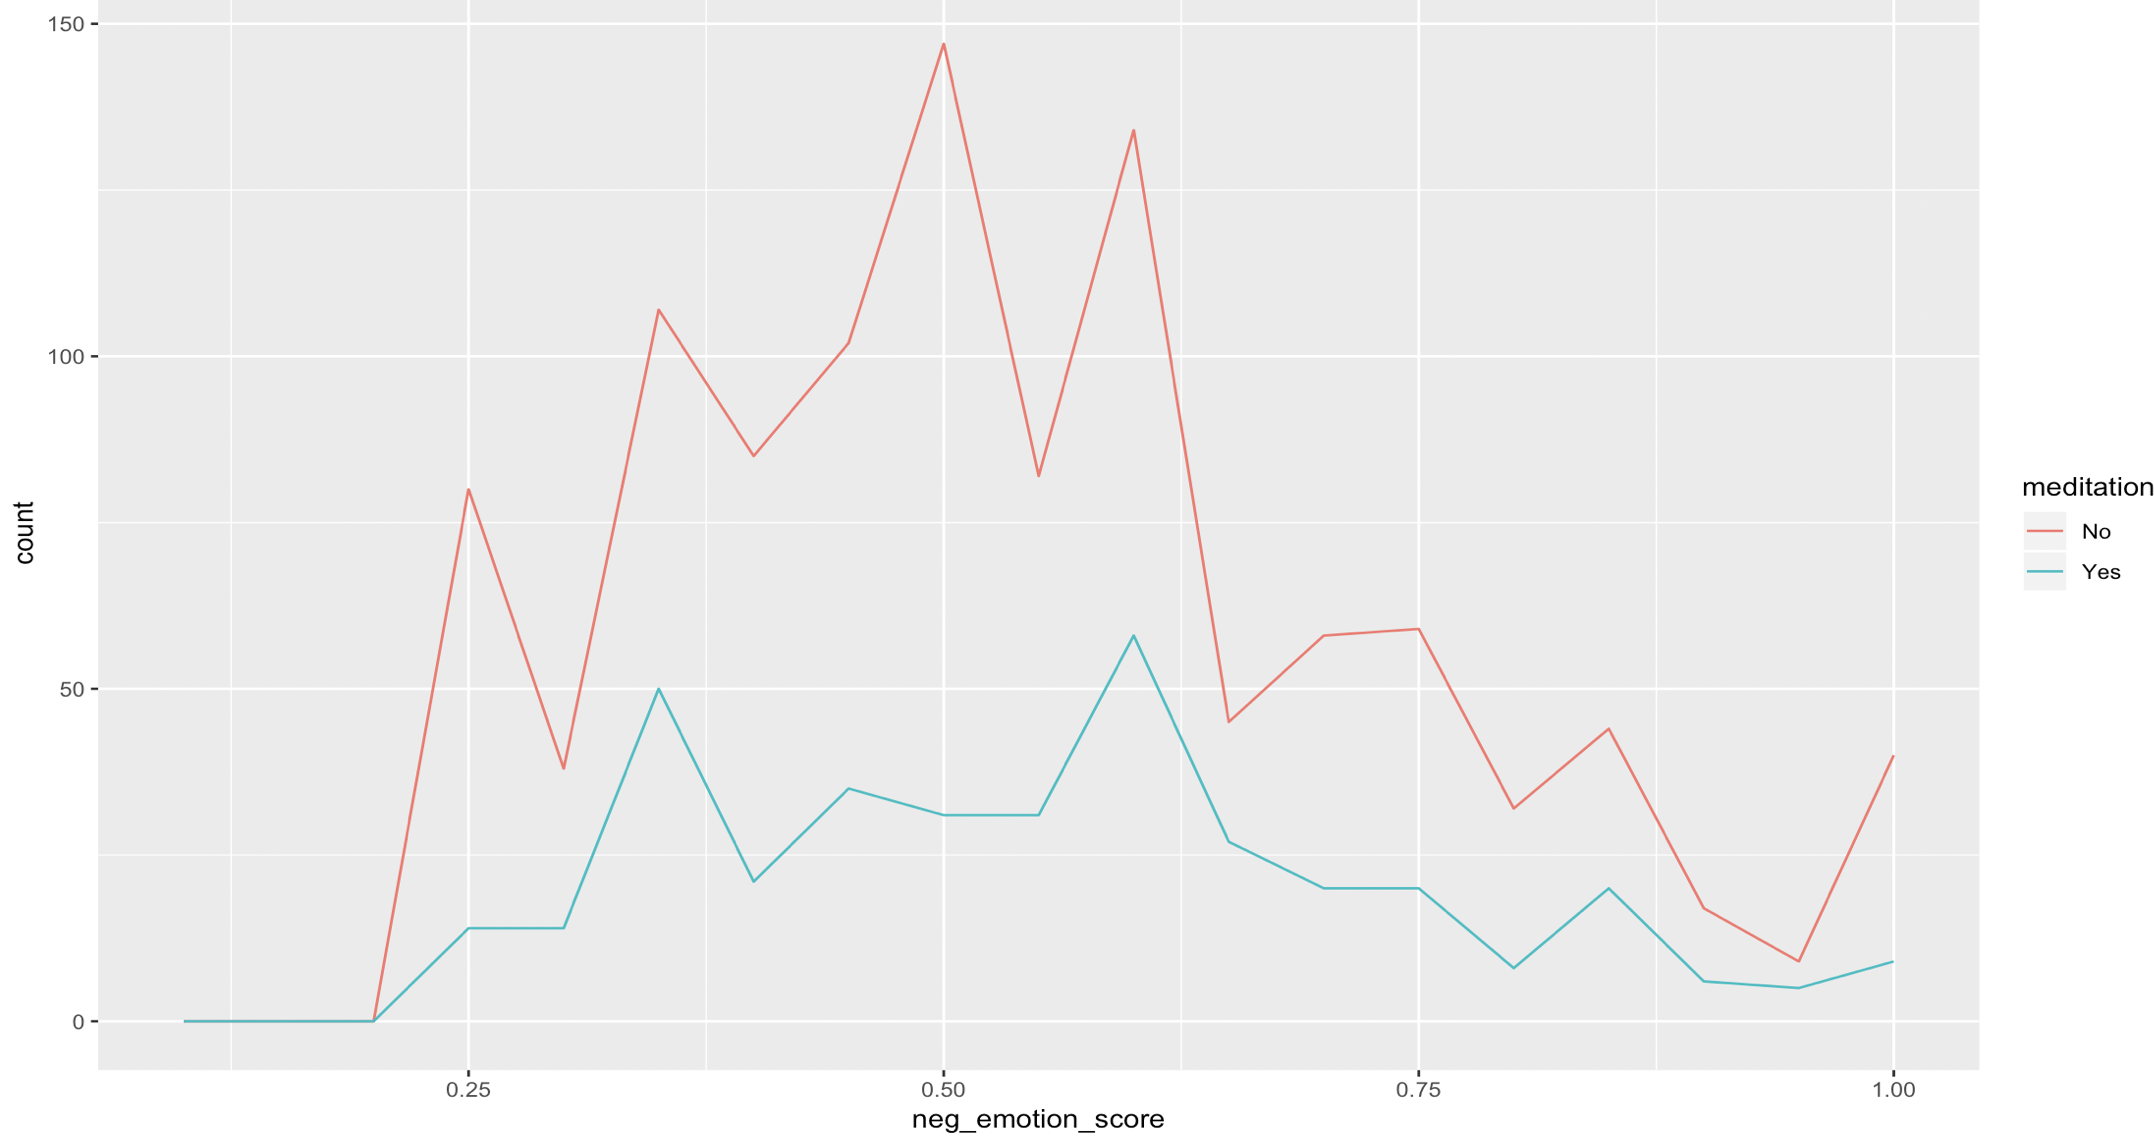
\includegraphics[scale=0.4]{medscore.png}
\caption{Meditation Vs Negative emotion score}
\label{fig:meditation}
\end{figure}

\begin{figure}[H]
\centering
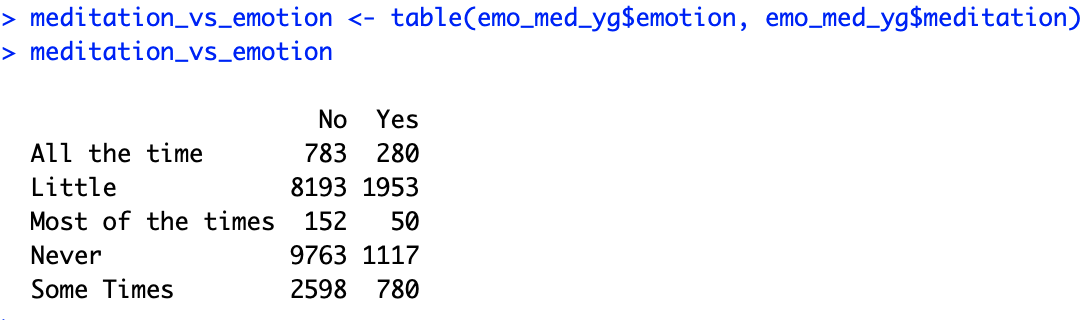
\includegraphics[scale=0.5]{table.png}
\caption{Frequency table}
\label{fig:frequency}
\end{figure}

\begin{figure}[H]
\centering
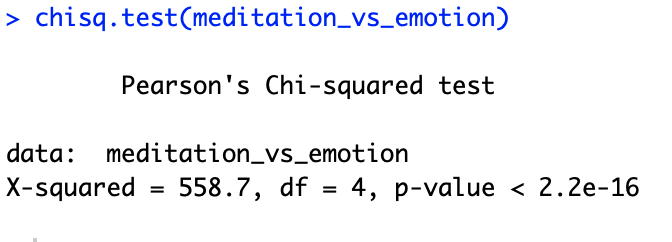
\includegraphics[scale=0.5]{chisqResult.png}
\caption{Chi Square test results}
\label{fig:chisq}
\end{figure}

\begin{figure}[H]
\centering
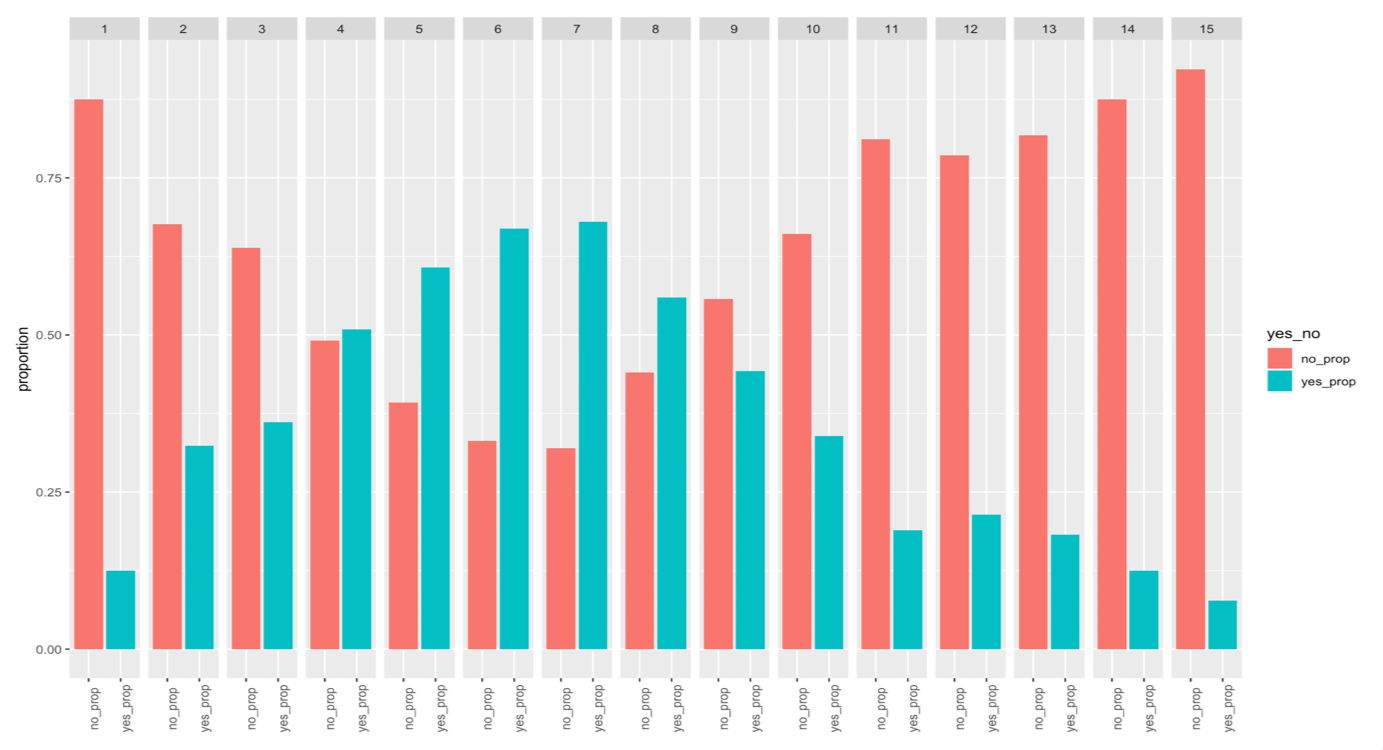
\includegraphics[scale = 0.4]{sleepIncome.png}
\caption{Proportion of people based on whether they have income from regular salary faceted by number of hours of sleep}
\label{fig:sleepvsincome}
\end{figure}

\begin{figure}[H]
\centering
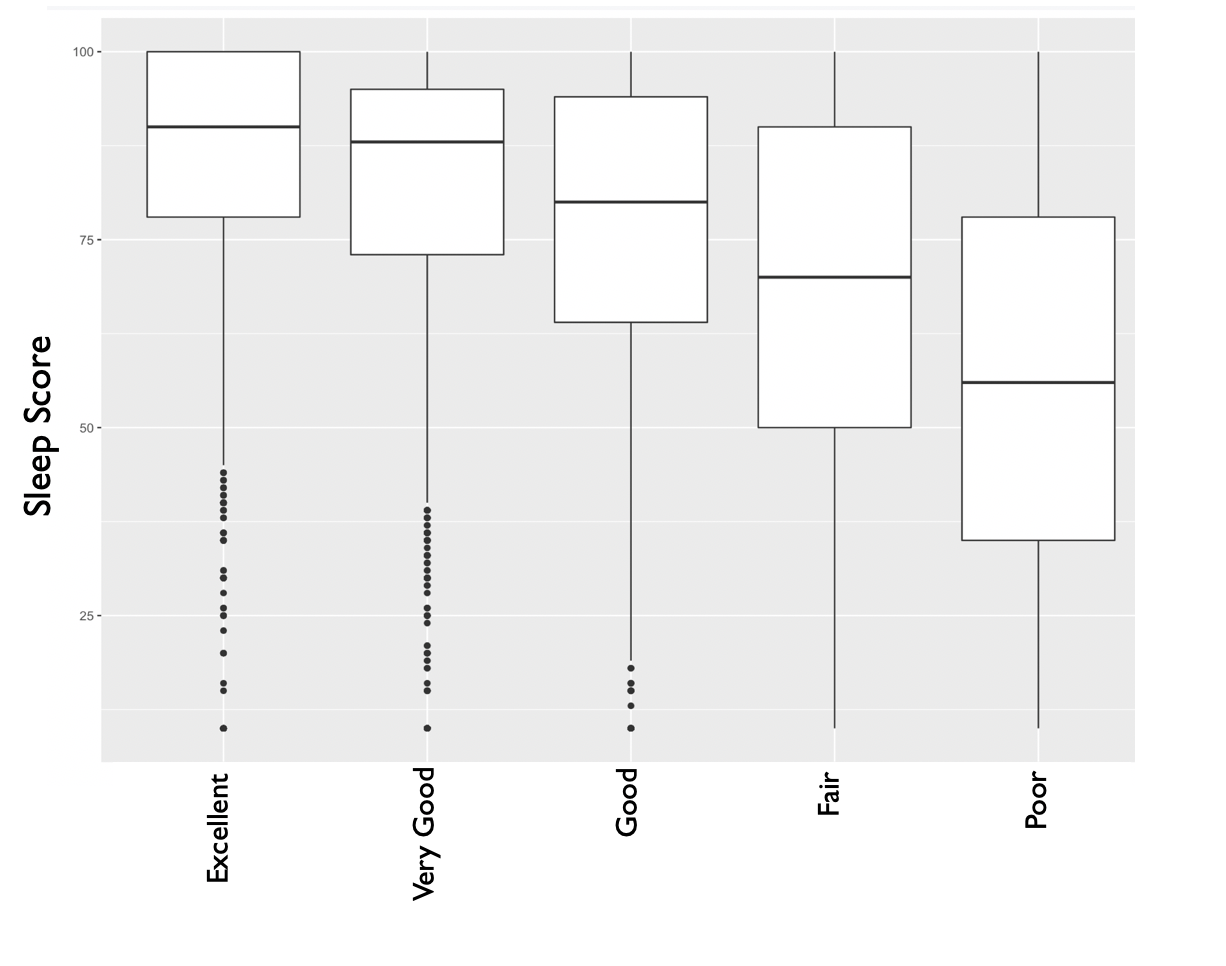
\includegraphics[scale = 0.4]{sleepHealth.png}
\caption{Sleep score Vs Health status}
\label{fig:sleepvshealth}
\end{figure}

\begin{figure}[H]
\centering
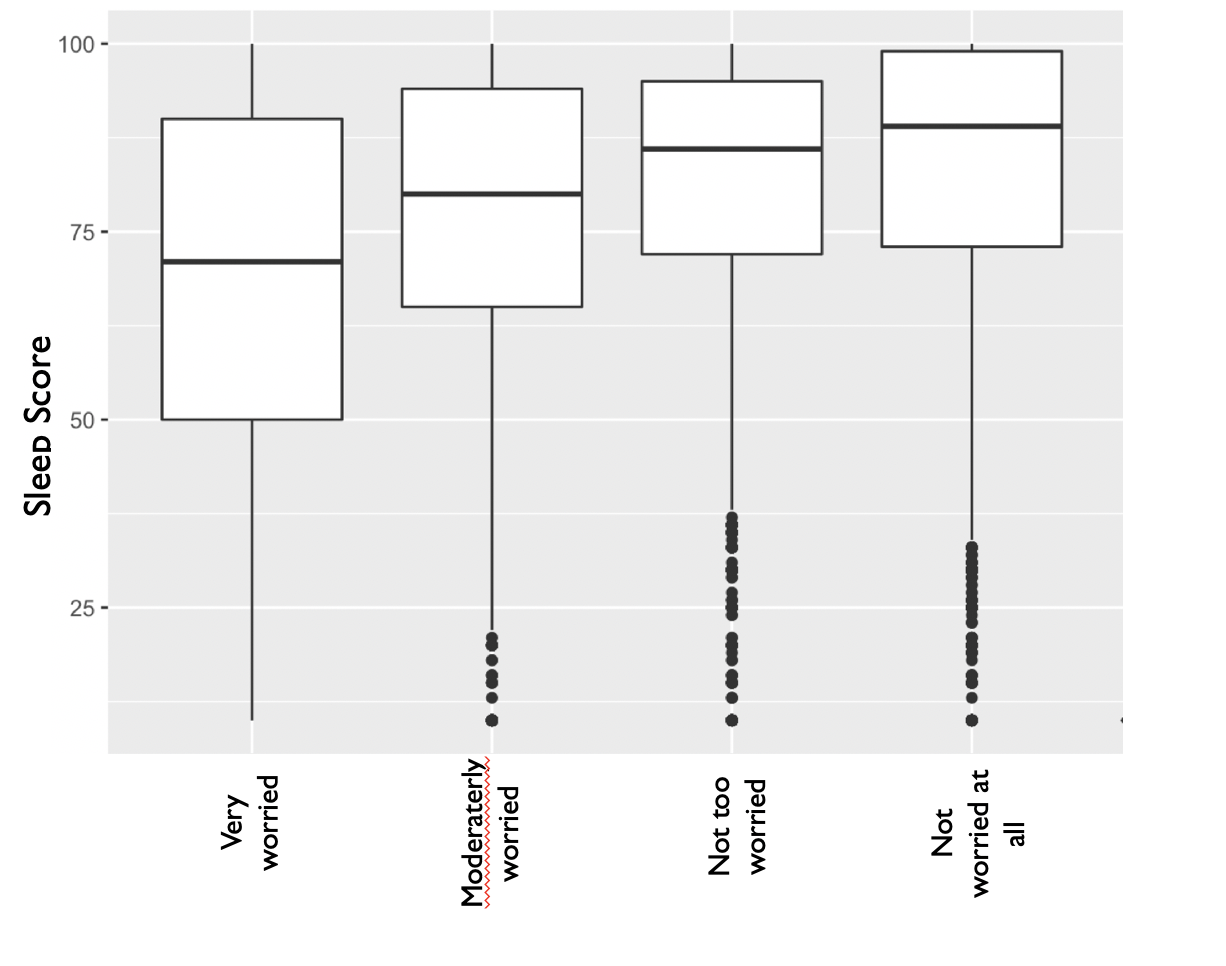
\includegraphics[scale = 0.4]{sleepHealthCare.png}
\caption{Sleep score Vs Affordability for normal health care}
\label{fig:sleepvshealthcare}
\end{figure}

\begin{figure}[H]
\centering
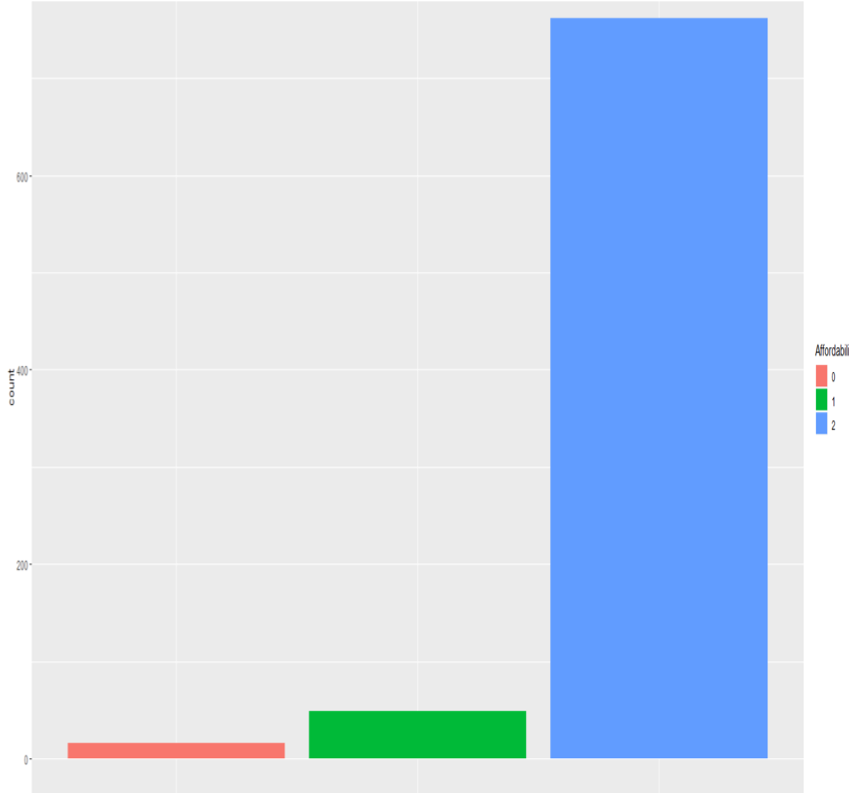
\includegraphics[scale=0.5]{dataimbalance.png}
\caption{Data Imbalance}
\label{fig:dataimbalance}
\end{figure}

\begin{figure}[H]
\centering
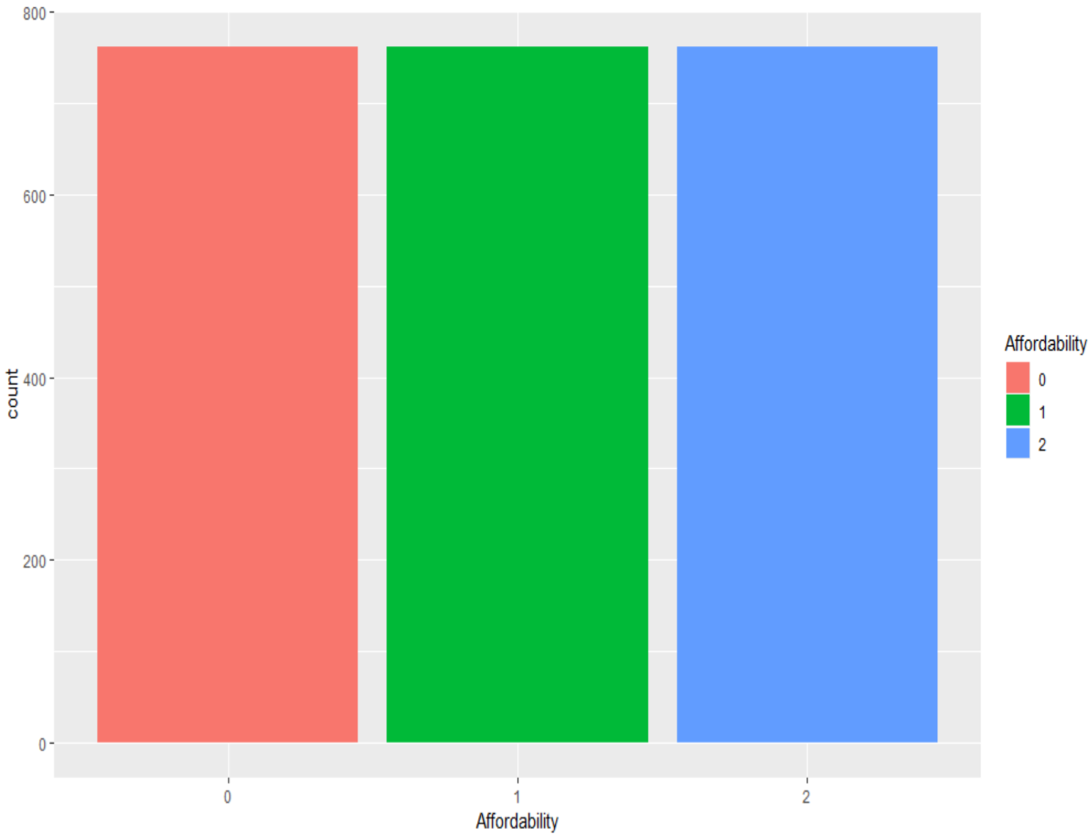
\includegraphics[scale=0.5]{balanced.png}
\caption{Balanced Data}
\label{fig:databalance}
\end{figure}

\begin{figure}[H]
\centering
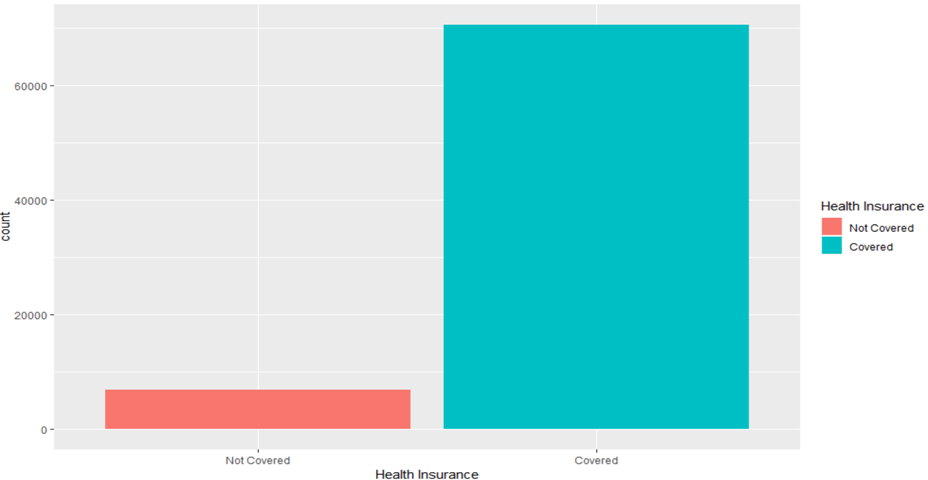
\includegraphics[scale=0.5]{insuredvsnot.png}
\caption{Insured Vs Not Insured}
\label{fig:insurance}
\end{figure}

\begin{figure}[H]
\centering
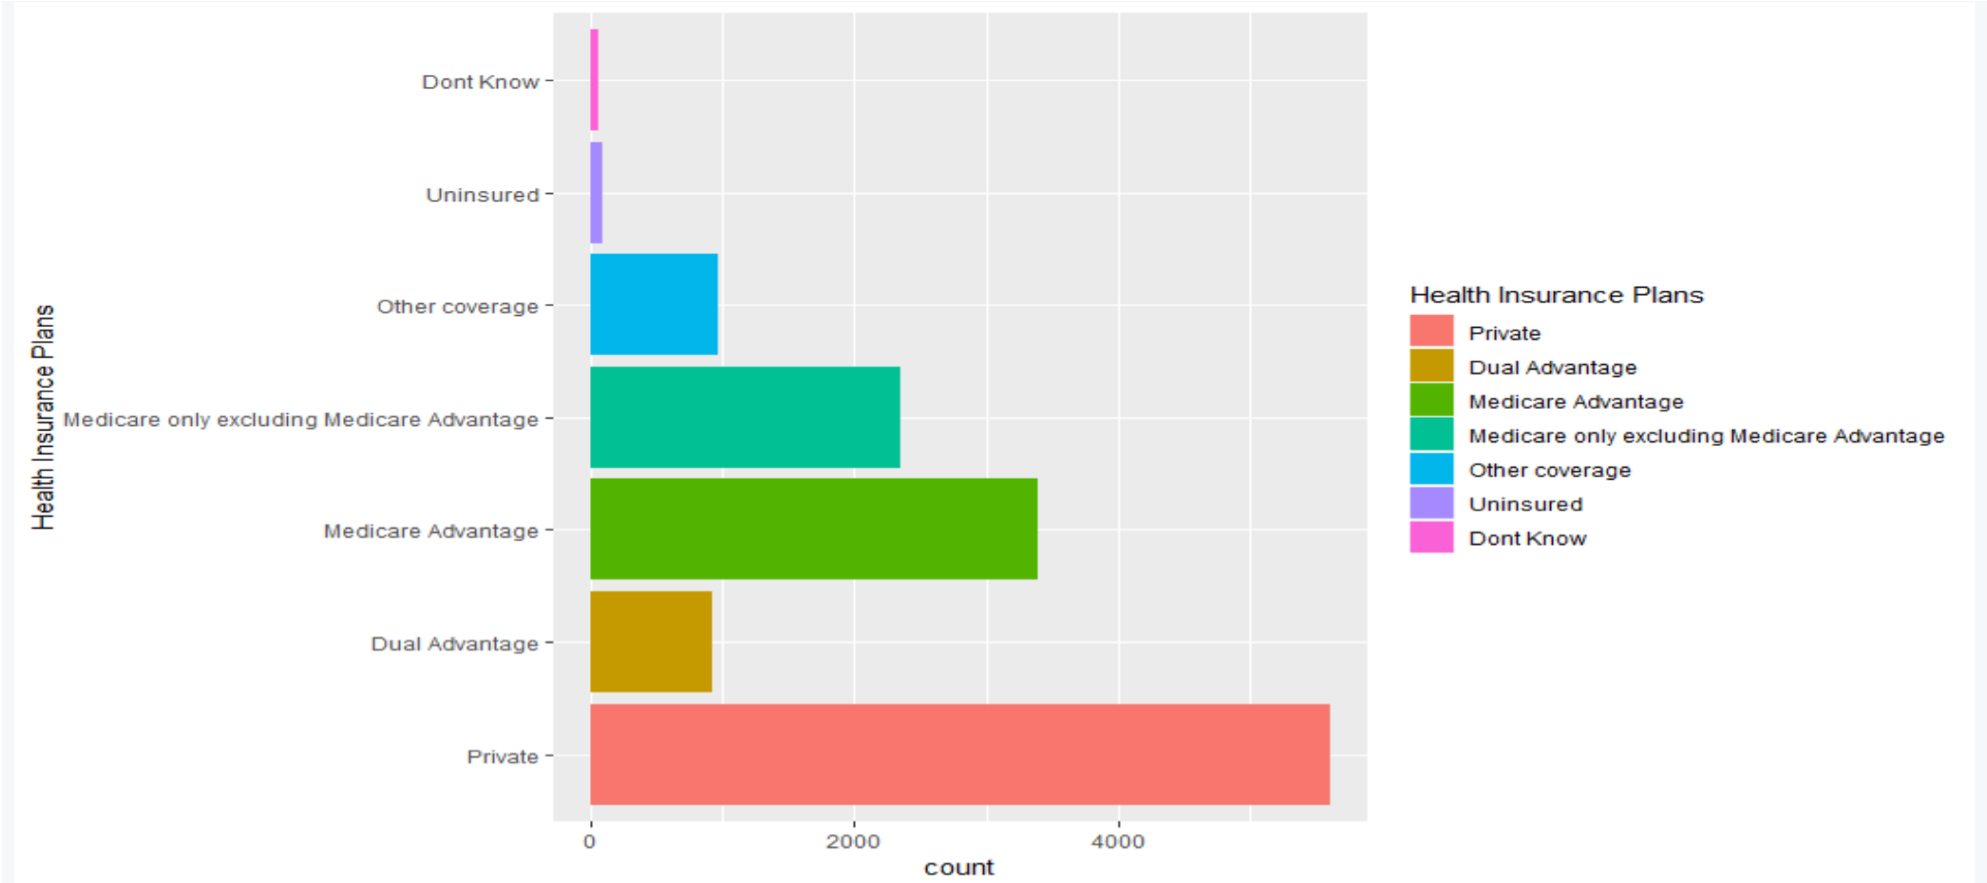
\includegraphics[scale=0.5]{privateplans.png}
\caption{Health care insurance plans}
\label{fig:privateplans}
\end{figure}

\begin{figure}[H]
\centering
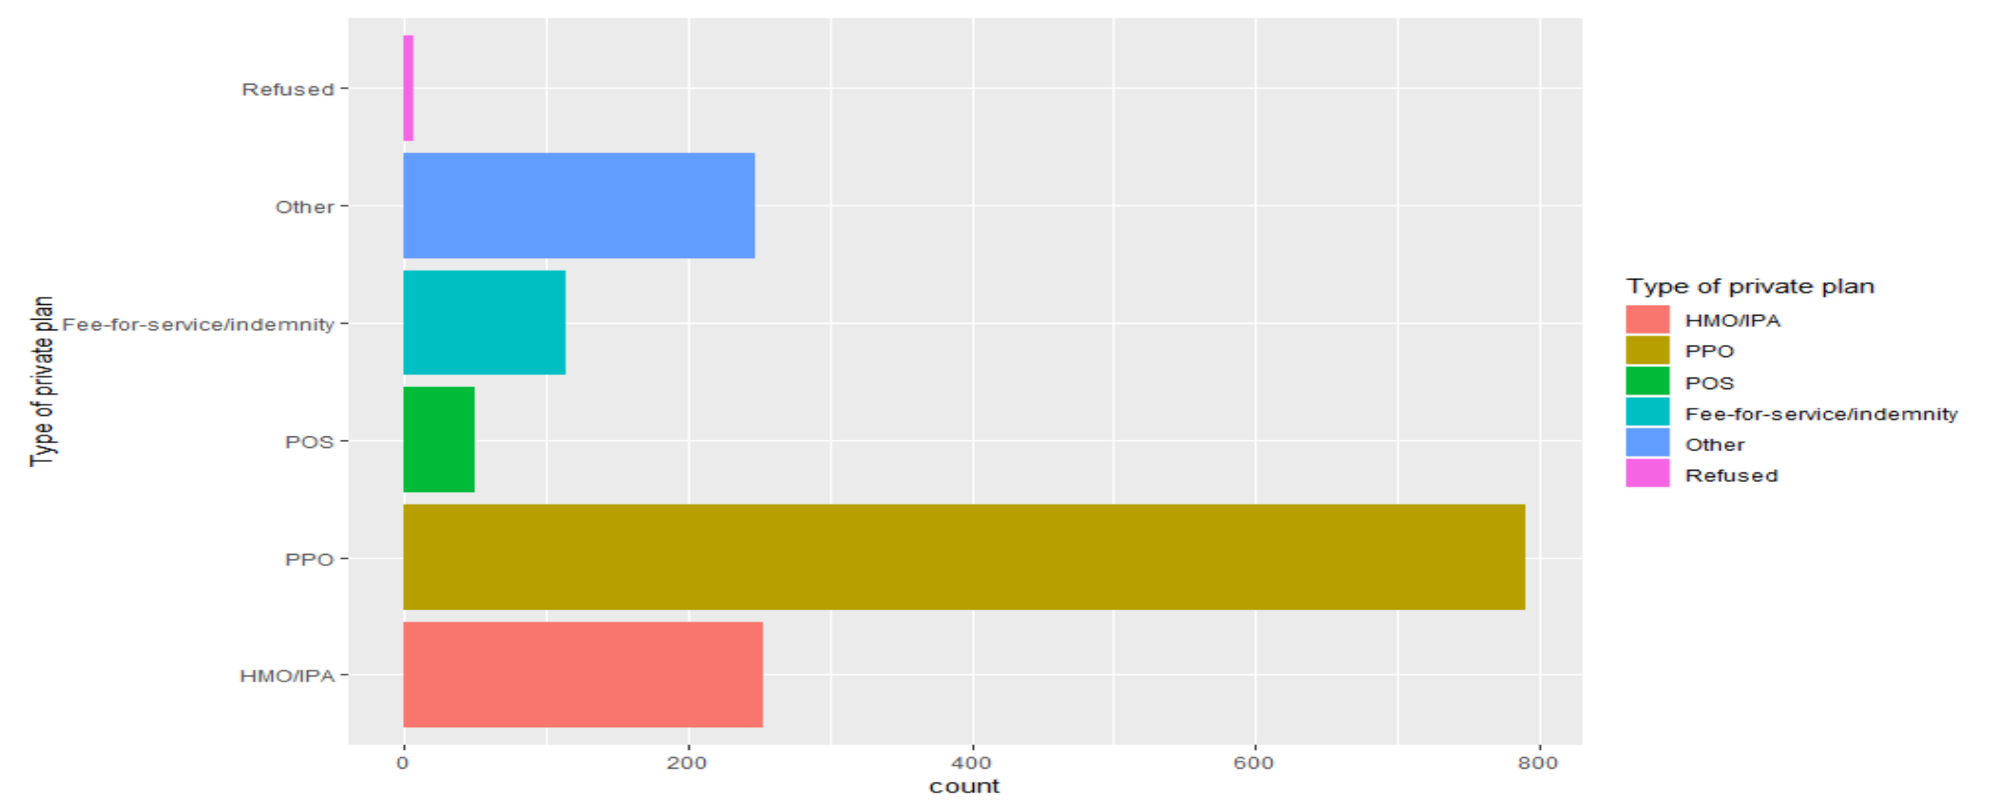
\includegraphics[scale=0.5]{ppo.png}
\caption{Private insurance plans}
\label{fig:ppo}
\end{figure}

\begin{figure}[H]
\centering
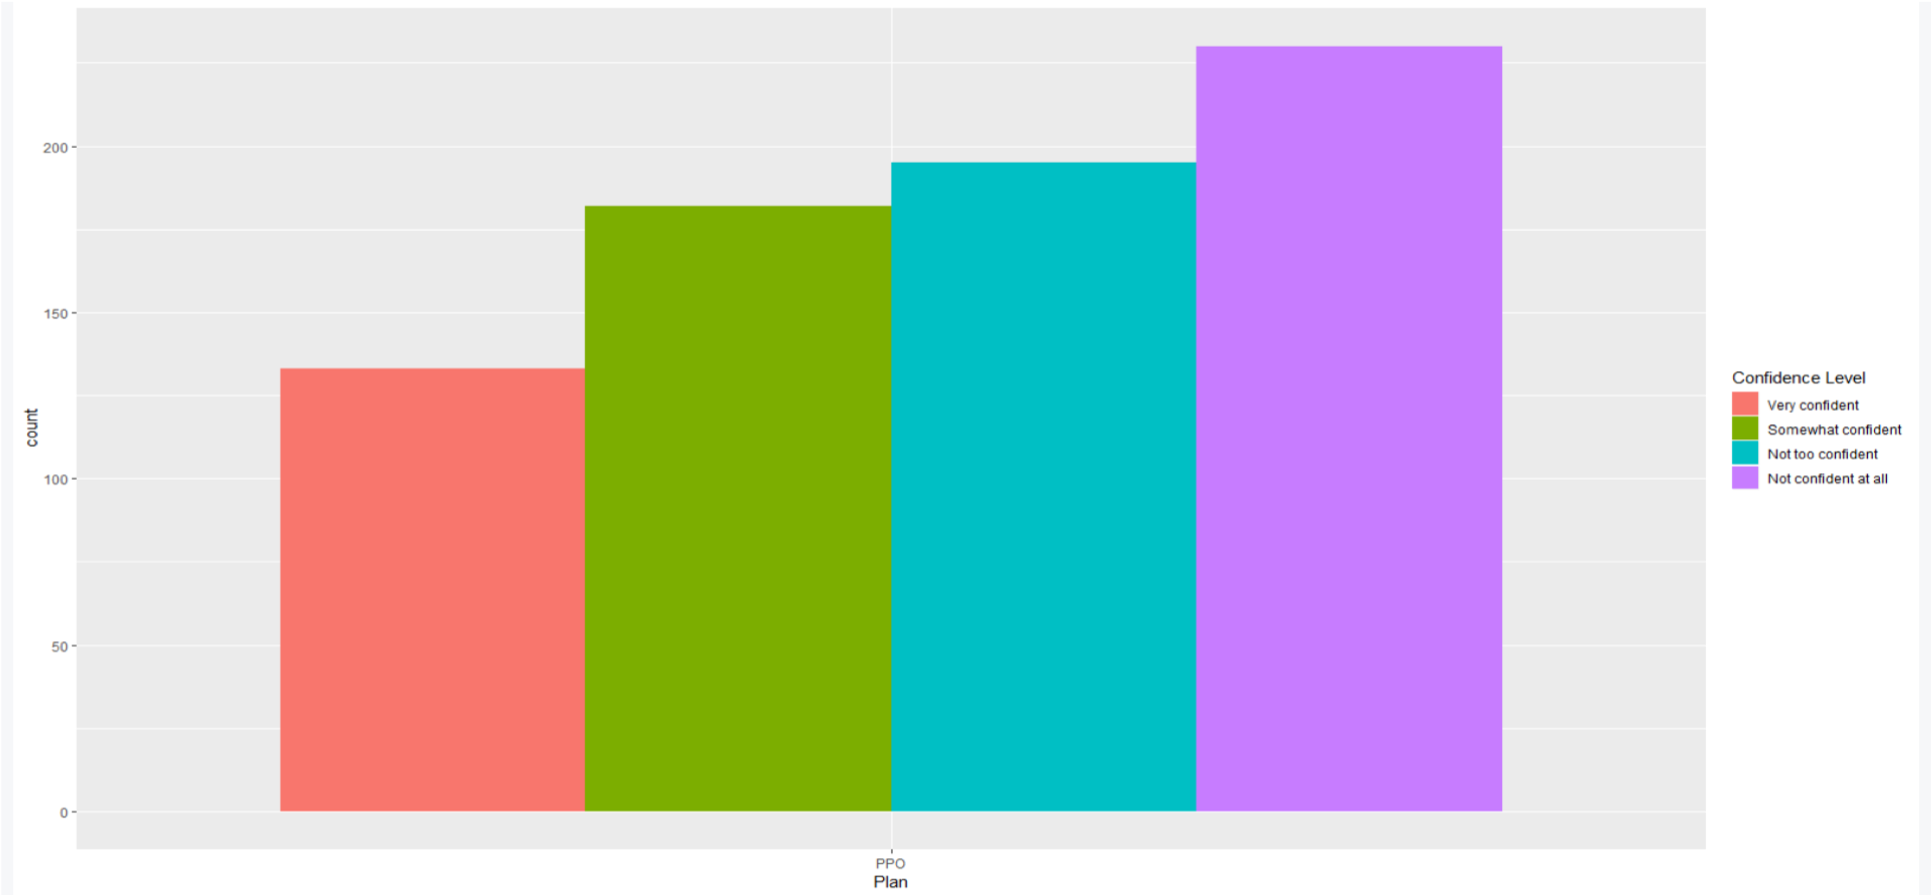
\includegraphics[scale=0.5]{notconfident.png}
\caption{Ability to afford other health care plans}
\label{fig:notconfident}
\end{figure}

\begin{figure}[H]
\centering
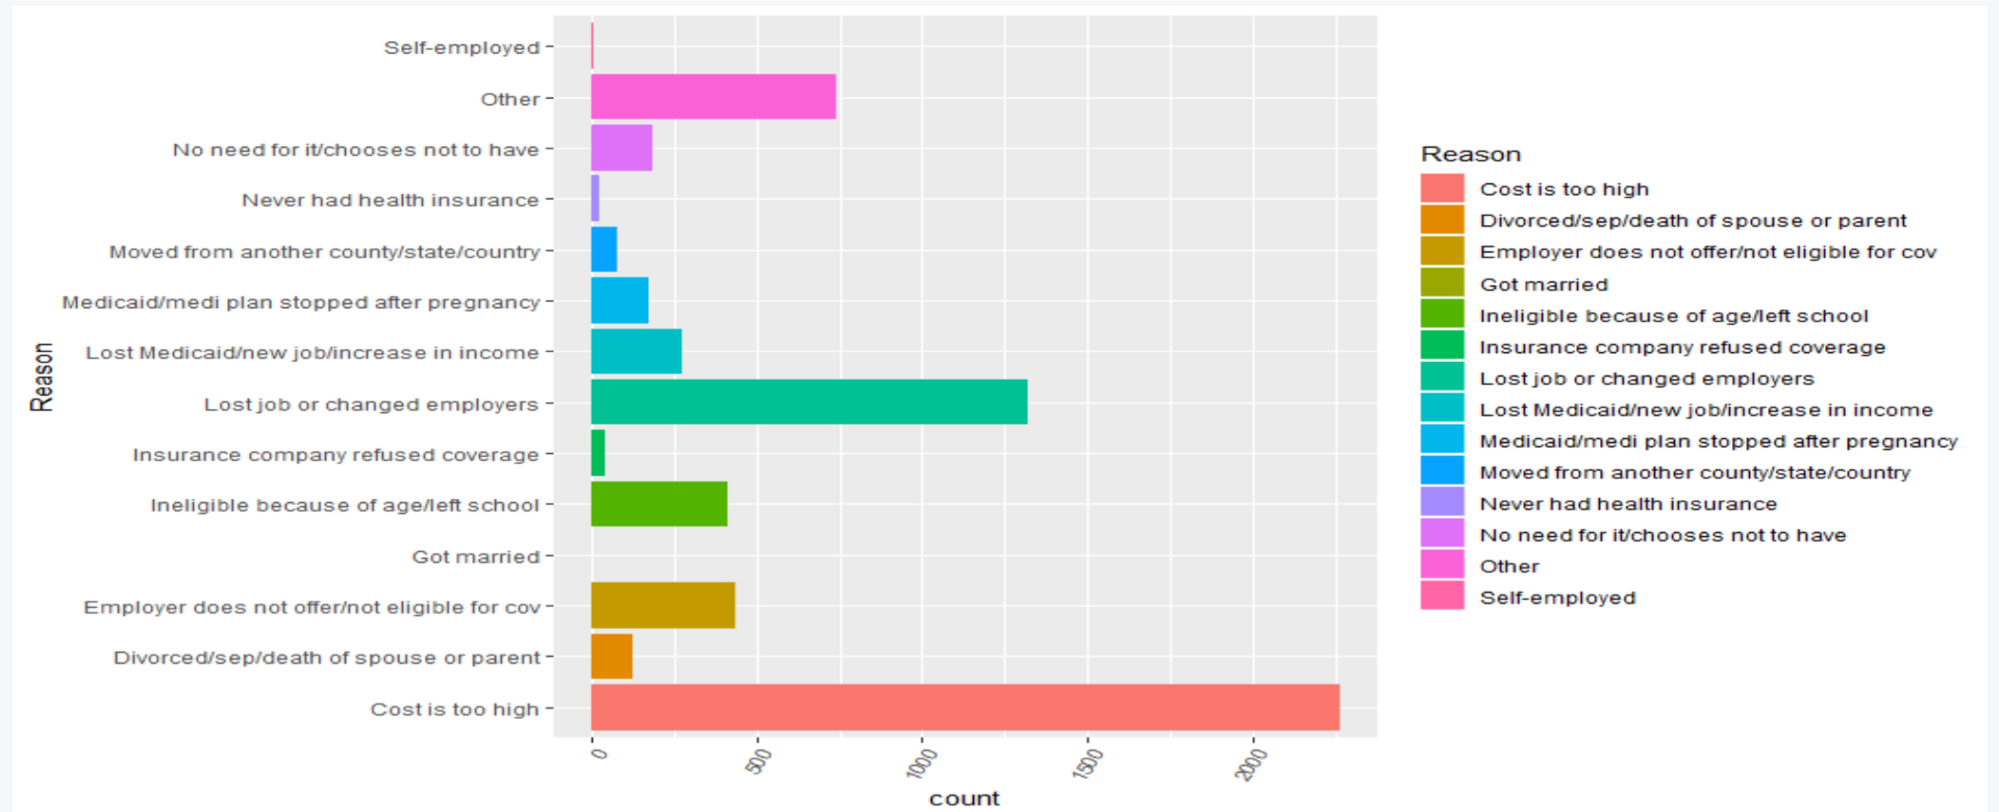
\includegraphics[scale=0.5]{reasonNotinsured.png}
\caption{Reasons for not being insured}
\label{fig:notinsured}
\end{figure}

\begin{figure}[H]
\centering
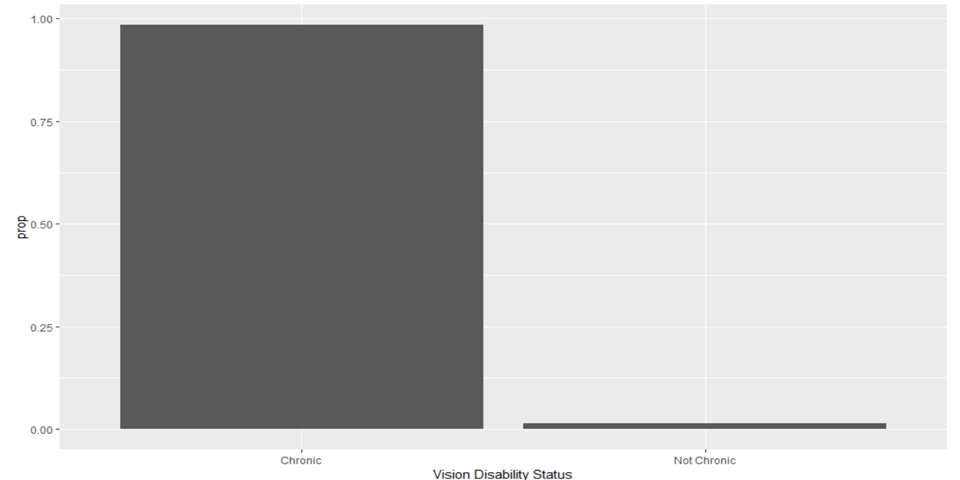
\includegraphics[scale=0.5]{visibility.png}
\caption{Current status of Visibility}
\label{fig:visibility}
\end{figure}

\begin{figure}[H]
\centering
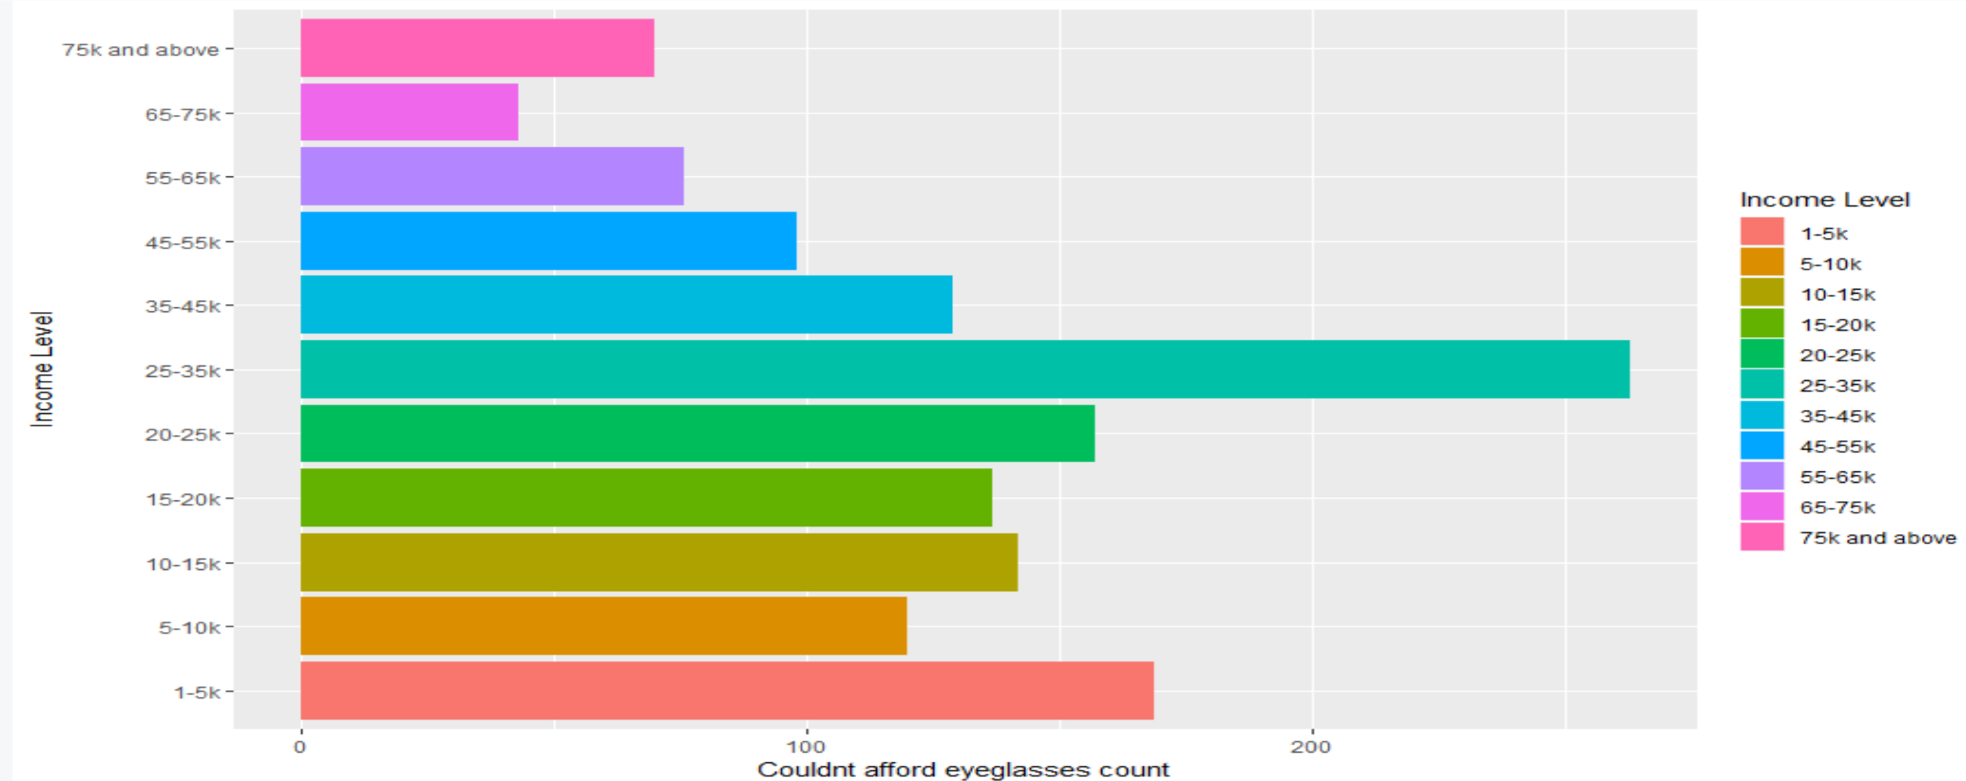
\includegraphics[scale=0.5]{eyeglass.png}
\caption{Income vs Ability to afford Eyeglasses}
\label{fig:eyeglass}
\end{figure}

\begin{figure}[H]
\centering
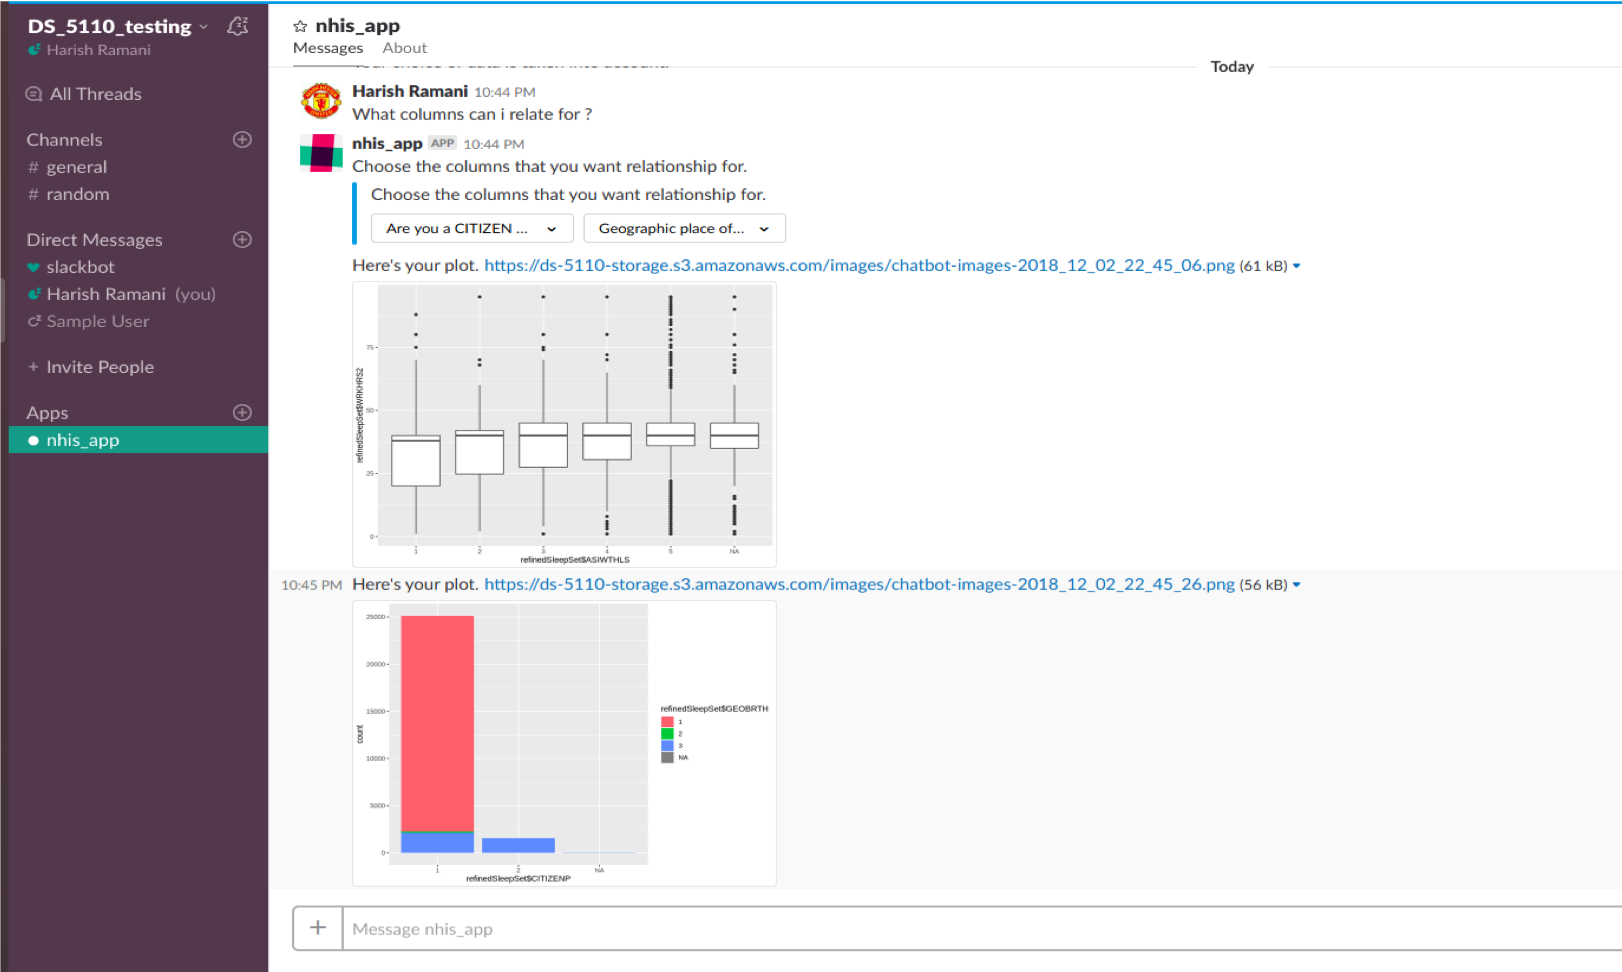
\includegraphics[scale=0.75]{slackbot.png}
\caption{Slack Bot}
\label{fig:slack}
\end{figure}

\end{document}